\documentclass[a4paper,12pt]{article}
 
\usepackage{pgfplots}
 
\pgfplotsset{compat = newest}
 
\begin{document}
 
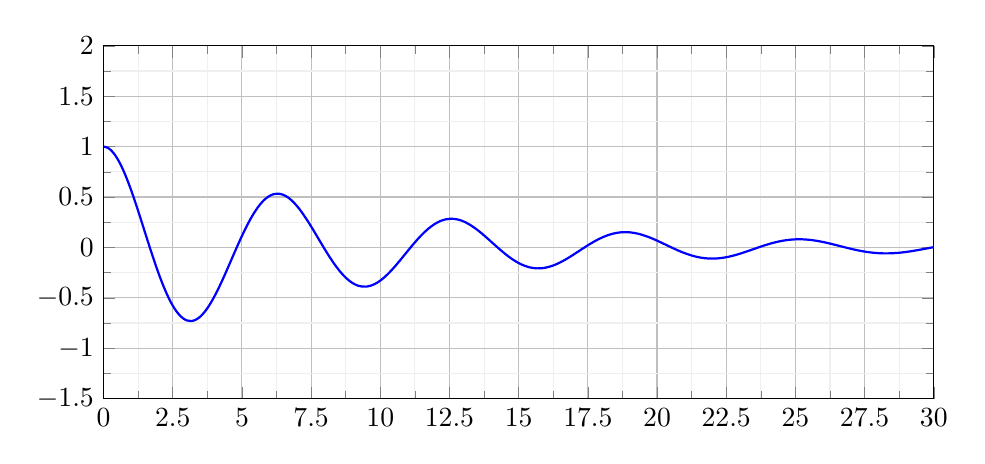
\begin{tikzpicture}
 
\begin{axis}[
    xmin = 0, xmax = 30,
    ymin = -1.5, ymax = 2.0,
    xtick distance = 2.5,
    ytick distance = 0.5,
    grid = both,
    minor tick num = 1,
    major grid style = {lightgray},
    minor grid style = {lightgray!25},
    width = \textwidth,
    height = 0.5\textwidth]
    \addplot[
        domain = 0:30,
        samples = 200,
        smooth,
        thick,
        blue,
    ] {exp(-x/10)*( cos(deg(x)) + sin(deg(x))/10 )};
\end{axis}
 
\end{tikzpicture}
 
\end{document}